
\serie{Fractions et partage}

\begin{exercice}[Un peu de vocabulaire]
Pour chaque figure, indique la fraction de la surface totale qui est colorée :
\begin{colenumerate}{3}
 \item 
 
 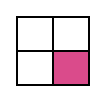
\includegraphics[width=1.3cm]{fraction1}
 \item 
 
 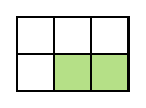
\includegraphics[width=2cm]{fraction2}
 \item 
 
 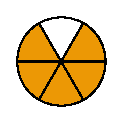
\includegraphics[width=1.6cm]{fraction3}
 \item 
 
 \quad 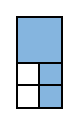
\includegraphics[width=0.8cm]{fraction4}
 \item 
 
 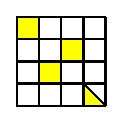
\includegraphics[width=1.6cm]{fraction5}
 \item 
 
 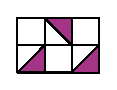
\includegraphics[width=1.5cm]{fraction6}
 \end{colenumerate}
\end{exercice}


\begin{exercice}
Dans quelle(s) figure(s) la surface colorée est‑elle égale au quart de la surface totale ?
\begin{colenumerate}{3}
 \item 
 
 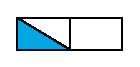
\includegraphics[width=1.9cm]{fraction7}
  \item 
 
 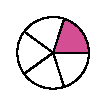
\includegraphics[width=1.3cm]{fraction8}
  \item 
 
 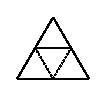
\includegraphics[width=1.3cm]{fraction9}
 \end{colenumerate}
\end{exercice}


\begin{exercice}[Drôles de partages]
Dans quelle(s) figure(s) la surface colorée est‑elle égale au quart de la surface totale ?
\begin{colenumerate}{2}
 \item 
 
 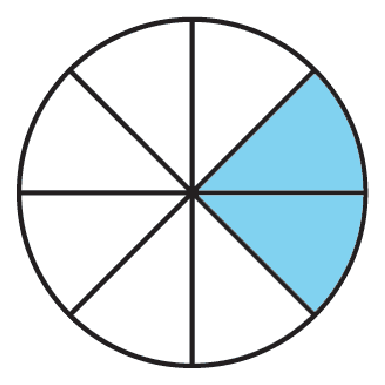
\includegraphics[width=2.1cm]{partage1}
  \item 
 
 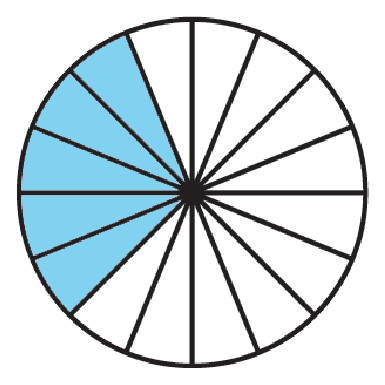
\includegraphics[width=2.1cm]{partage2}
   \item 
 
 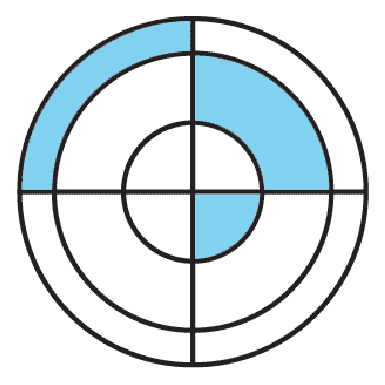
\includegraphics[width=2.1cm]{partage3}
   \item 
 
 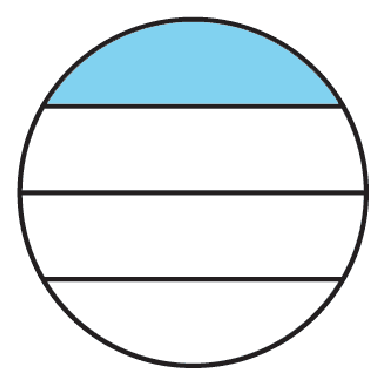
\includegraphics[width=2.1cm]{partage4}
 \end{colenumerate}
\end{exercice}


\begin{exercice}[Avec des quadrilatères]
\begin{enumerate}
  \item Trace un carré de côté 5 cm et colorie trois quarts de sa surface.
  \item Trace un rectangle de largeur 3 cm et de longueur 7 cm. Colorie $\dfrac{7}{21}$ de sa surface.
  \item Trace un carré de côté 3 cm et colorie un sixième de sa surface.
 \end{enumerate}
\end{exercice}


\begin{exercice}[Avec un segment]
\begin{enumerate}
 \item En utilisant le quadrillage de ton cahier, reproduis le segment suivant : \label{NbsRatio_acti10}
 
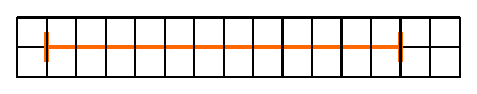
\includegraphics[width=7.9cm]{segment_fraction}
 \item Construis un segment dont la longueur par rapport à celle du segment de la question \ref{NbsRatio_acti10} est :
 \begin{colitemize}{3}
  \item $\dfrac{1}{4}$ ;
  \item $\dfrac{1}{6}$ ;
  \item $\dfrac{5}{4}$.
  \end{colitemize}
 \end{enumerate}
\end{exercice}

%%%%%%%%%%%%%%%%%%%%%%%%%%%%%%%%%%%%%%%%%%%%%%%%%%%%%%%%%%%%%%%%%%%%%%%%

\serie{Différentes écritures}

\begin{exercice}
Donne une écriture fractionnaire des nombres suivants :
\begin{colenumerate}{2}
 \item une demie ;
 \item cinq douzièmes ;
 \item deux tiers ;
 \item sept demis ;
 \item trois quarts ;
 \item cent dix-neuvièmes ;
 \item moins un quart ;
 \item moins trois septièmes.
 \end{colenumerate}
\end{exercice}


\begin{exercice}
Donne une écriture décimale des nombres :
\begin{colenumerate}{2}
 \item deux centièmes ;
 \item quarante dixièmes ;
 \item trois dixièmes ;
 \item cinq-cent millièmes ;
 \item cinq cent‑millièmes ;
 \item neuf tiers ;
 \item moins vingt-deux \newline dixièmes ;
 \item moins cent vingt-trois \newline millièmes.
 \end{colenumerate}
\end{exercice}


\begin{exercice}
Détermine la fraction dont le dénominateur est le numérateur de $\dfrac{41}{17}$ et dont le numérateur est le triple du dénominateur de $\dfrac{53}{9}$.
\end{exercice}


\begin{exercice}
Recopie et complète par deux entiers consécutifs les encadrements suivants :
\begin{colenumerate}{2}
 \item $\ldots < \dfrac{36}{10} < \ldots$ ;
 \item $\ldots < \dfrac{2}{7} < \ldots$ ;
 \item $\ldots < \dfrac{11}{3} < \ldots$ ;
 \item $\ldots < \dfrac{49}{8} < \ldots$ ;
 \end{colenumerate}
\end{exercice}


\begin{exercice}
Recopie et complète par deux entiers consécutifs les encadrements suivants :
\begin{colenumerate}{2}
 \item $\ldots < \dfrac{- 12}{10} < \ldots$ ;
 \item $\ldots < \dfrac{- 18}{7} < \ldots$ ;
 \item $\ldots < \dfrac{-44}{3} < \ldots$ ;
 \item $\ldots < \dfrac{- 35}{8} < \ldots$ ;
 \end{colenumerate}
\end{exercice}


\begin{exercice}
Parmi les fractions suivantes, indique celles qui sont égales à des nombres entiers, puis celles qui sont inférieures à 1 : \\[0.3em]
$\dfrac{42}{10}$ ; $\dfrac{8}{2}$ ; $\dfrac{36}{5}$ ; $\dfrac{1}{6}$ ; $\dfrac{27}{3}$ ; $\dfrac{126}{9}$ ; $\dfrac{87}{2}$ ; $\dfrac{132}{4}$ ; $\dfrac{4}{3}$ ; $\dfrac{33}{42}$.
\end{exercice}


\begin{exercice}
Recopie et complète :
\begin{colenumerate}{3}
 \item $\dfrac{\ldots \ldots}{9} = 1$ ;
 \item $5 = \dfrac{\ldots \ldots}{8}$ ;
 \item $0 = \dfrac{\ldots \ldots}{6}$ ;
 \item $\dfrac{\ldots \ldots}{2} = 4,5$ ;
 \item $\dfrac{1}{\ldots \ldots} = 0,001$ ;
 \item $2,5 = \dfrac{\ldots \ldots}{4}$.
 \end{colenumerate}
\end{exercice}


\begin{exercice}
On considère le quotient $12 : 5$ :
\begin{enumerate}
 \item Donne une écriture fractionnaire de ce quotient. Quel est le numérateur ? Le dénominateur ? \label{NbsRatio_acti11}
 \item Donne une écriture décimale de ce quotient. \label{NbsRatio_acti12}
 \item Reprends les questions \ref{NbsRatio_acti11} et \ref{NbsRatio_acti12} en considérant maintenant le quotient $7 : 8$.
 \end{enumerate}
\end{exercice}


\begin{exercice}
Donne l'écriture décimale de chaque nombre :
\begin{colenumerate}{5}
 \item $\dfrac{1}{8}$ ; 
 \item $\dfrac{46}{5}$ ; 
 \item $\dfrac{56}{70}$ ; 
 \item $\dfrac{11}{16}$ ; 
 \item $\dfrac{153}{12}$.
 \end{colenumerate}
\end{exercice}


%%%%%%%%%%%%%%%%%%%%%%%%%%%%%%%%%%%%%%%%%%%%%%%%%%%%%%%%%%%%%%%%%%%%%%%%

\serie{Demi‑droite graduée}

\begin{exercice}
Donne, sous forme d'une fraction, l'abscisse de chacun des points $A$, $B$ et $C$ placés sur la demi‑droite graduée ci‑dessous :
\begin{center} 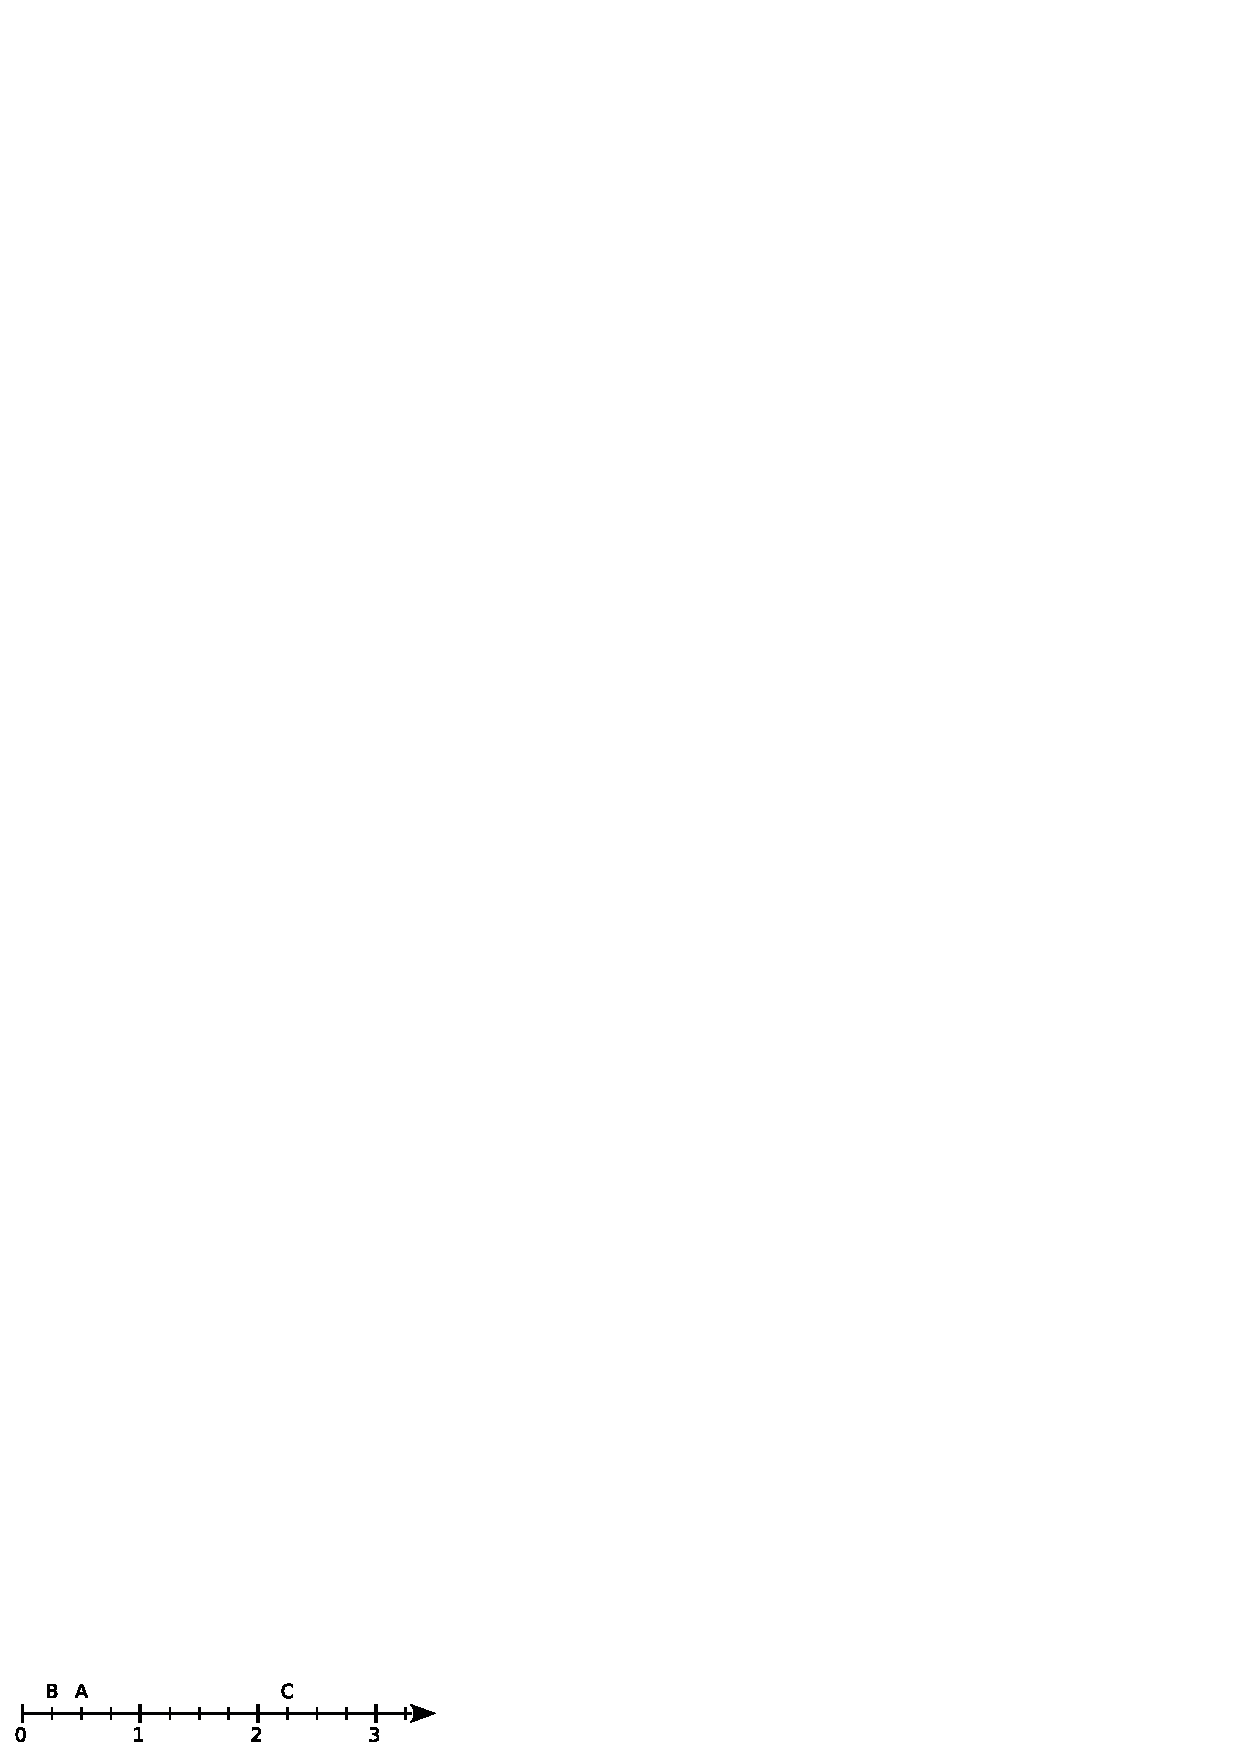
\includegraphics[width=8cm]{dd_BAC03} \end{center}
Donne, sous forme d'une fraction, l'abscisse de chacun des points $R$, $S$ et $T$ placés sur la demi‑droite graduée ci‑dessous :
\begin{center} 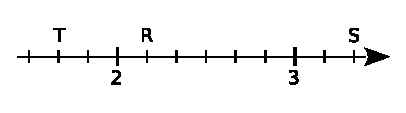
\includegraphics[width=7cm]{dd_TRS23} \end{center}
\end{exercice}


\begin{exercice}
Trace une demi‑droite graduée en prenant 10 cm pour une unité et place les points $M$, $N$, $P$ et $Q$ d'abscisses respectives $\dfrac{3}{10}$ ; 0,7 ; $\dfrac{12}{10}$ et $\dfrac{2}{5}$.
\end{exercice}


\begin{exercice}
Trace une demi‑droite graduée en prenant 10 cm pour une unité et place les points $M$, $N$, $P$ et $Q$ d'abscisses respectives $- \dfrac{7}{10}$ ; $- 0,3$ ; $- \dfrac{2}{10}$ et $- \dfrac{8}{5}$.
\end{exercice}


\begin{exercice}
Trace une demi‑droite graduée en prenant une unité de 3 cm. Place les nombres $\dfrac{5}{3}$ ; $\dfrac{7}{3}$ ; 0,2 ; $\dfrac{4}{5}$ ; $\dfrac{17}{5}$ et 1,5.
\end{exercice}


\begin{exercice}
En choisissant judicieusement la longueur d'une graduation, place précisément sur une demi‑droite graduée les points $A$, $B$, $C$, $D$ et $E$ d'abscisses respectives $\dfrac{5}{12}$, $\dfrac{7}{6}$, $\dfrac{2}{3}$, $\dfrac{3}{2}$ et $\dfrac{5}{4}$.
\end{exercice}


\begin{exercice}
Trace une demi‑droite graduée en prenant 7 cm pour une unité et place les points $E$, $F$ et $G$ d'abscisses respectives $\dfrac{2}{7}$, $1 + \dfrac{3}{7}$ et $1 - \dfrac{4}{7}$.
\end{exercice}


\begin{exercice}
Place précisément sur une demi‑droite graduée les points $U$, $V$ et $W$ d'abscisses respectives $2 + \dfrac{1}{3}$, $6 - \dfrac{2}{3}$ et $3 + \dfrac{4}{3}$.
\end{exercice}

%%%%%%%%%%%%%%%%%%%%%%%%%%%%%%%%%%%%%%%%%%%%%%%%%%%%%%%%%%%%%%%%%%%%%%%%

\serie{Amplifier, simplifier, égalités}

\begin{exercice}[Partage de disques]
En t'inspirant des schémas ci-dessous, écris des égalités de fractions :
\begin{colenumerate}{3}
 \item
 
 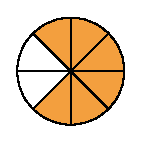
\includegraphics[width=1.5cm]{disque1}
 \item
 
 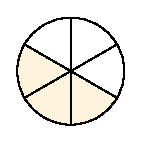
\includegraphics[width=1.5cm]{disque2}
 \item
 
 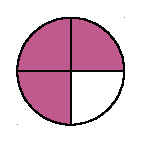
\includegraphics[width=1.5cm]{disque3}
 \item
 
 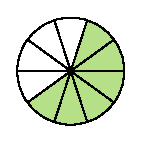
\includegraphics[width=1.5cm]{disque4}
 \item
 
 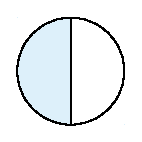
\includegraphics[width=1.5cm]{disque5}
 \item
 
 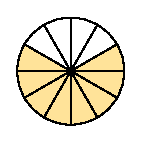
\includegraphics[width=1.5cm]{disque6}
 \item
 
 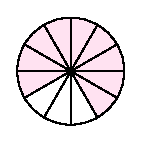
\includegraphics[width=1.5cm]{disque7}
 \item
 
 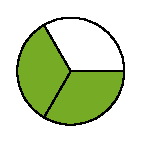
\includegraphics[width=1.5cm]{disque8}
 \item
 
 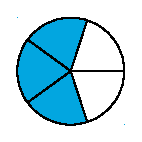
\includegraphics[width=1.5cm]{disque9}
 \end{colenumerate}
\end{exercice}


\begin{exercice}[Numérateur ou dénominateur fixé]
Recopie et complète :
\begin{colenumerate}{2}
 \item $\dfrac{4}{5} = \dfrac{4 \cdot \ldots}{5 \cdot \ldots} = \dfrac{\ldots}{15}$ ;
 \vspace{0.3cm}
 \item $\dfrac{2}{7} = \dfrac{2 \cdot \ldots}{7 \cdot \ldots} = \dfrac{\ldots}{56}$ ;
 \vspace{0.3cm}
 \item $\dfrac{4}{3} = \dfrac{4 \cdot \ldots}{3 \cdot \ldots} = \dfrac{\ldots}{9}$ ;
 \item $\dfrac{15}{18} = \dfrac{\ldots \cdot \ldots}{6 \cdot \ldots} = \dfrac{\ldots}{6}$ ;
 \item $\dfrac{7}{14} = \dfrac{1 \cdot \ldots}{\ldots \cdot \ldots} = \dfrac{1}{\ldots}$ ;
 \item $\dfrac{12}{20} = \dfrac{\ldots \cdot \ldots}{2 \cdot \ldots} = \dfrac{\ldots}{\ldots}$.
 \end{colenumerate}
\end{exercice}


\begin{exercice}[Numérateur ou dénominateur fixé (bis)]
Recopie et complète :
\begin{colenumerate}{3}
 \item $\dfrac{7}{3} = \dfrac{\ldots}{6}$ ;
 \vspace{0.3cm}
 \item $\dfrac{1}{4} = \dfrac{2}{\ldots}$ ;
 \item $\dfrac{7}{5} = \dfrac{21}{\ldots}$ ;
 \item $\dfrac{3}{4} = \dfrac{\ldots}{100}$ ;
 \item $\dfrac{12}{8} = \dfrac{\ldots}{4}$ ;
 \item $\dfrac{100}{80} = \dfrac{25}{\ldots}$.
 \end{colenumerate}
\end{exercice}


\begin{exercice}[Avec une étape]
Recopie et complète :
\begin{colenumerate}{2}
 \item $\dfrac{10}{6} = \dfrac{\ldots}{3} = \dfrac{25}{\ldots}$ ;
 \vspace{0.3cm}
 \item $\dfrac{12}{15} = \dfrac{\ldots}{5} = \dfrac{8}{\ldots}$ ;
 \vspace{0.3cm}
 \item $\dfrac{27}{18} = \dfrac{\ldots}{2} = \dfrac{15}{\ldots}$ ;
 \item $\dfrac{45}{60} = \dfrac{3}{\ldots} = \dfrac{\ldots}{28}$ ;
 \item $\dfrac{26}{65} = \dfrac{\ldots}{5} = \dfrac{\ldots}{10}$ ;
 \item $\dfrac{49}{42} = \dfrac{7}{\ldots} = \dfrac{\ldots}{72}$.
 \end{colenumerate}
\end{exercice}


\begin{exercice}[Égalités de fractions]
Dans chaque cas, indique, en justifiant, si les fractions données sont égales :
\begin{colenumerate}{2}
 \item $\dfrac{2}{3}$ et $\dfrac{10}{15}$ ;
 \vspace{0.3cm}
 \item $\dfrac{12}{8}$ et $\dfrac{36}{16}$ ;
 \item $\dfrac{12}{15}$ et $\dfrac{4}{5}$ ;
 \item $\dfrac{2}{3}$ et $\dfrac{4}{9}$.
 \end{colenumerate}
\end{exercice}


\begin{exercice}[À la recherche des nombres égaux]
Trouve, parmi les nombres suivants, ceux qui sont égaux :
\begin{colitemize}{3}
 \item $A = \dfrac{7}{4}$ ;
  \vspace{0.2cm}
 \item $B = \dfrac{3}{7}$ ;
   \vspace{0.2cm}
 \item $C = \dfrac{12}{5}$ ;
   \vspace{0.2cm}
 \item $D = \dfrac{9}{49}$ ;
   \vspace{0.2cm}
 \item $E = \dfrac{3}{2}$ ;
   \vspace{0.2cm}
 \item $F = \dfrac{33}{100}$ ;
 \item $G = \dfrac{28}{16}$ ;
 \item $H = \dfrac{1}{3}$ ;
 \item $I = \dfrac{21}{49}$ ;
 \item $J = \dfrac{14}{8}$ ;
 \item $K = 1,5$ ;
 \item $L = \dfrac{18}{12}$ ;
 \item $M = \dfrac{1,2}{0,5}$ ;
 \item $N = \dfrac{15}{10}$ ;
 \item $P = 0,33$ ;
 \item $Q = \dfrac{45}{105}$.
 \end{colitemize}
\end{exercice}


\begin{exercice}[Intrus]
Dans chacune des listes de fractions suivantes se cache un intrus. Trouve-le en justifiant.
\begin{enumerate}
 \item $\dfrac{80}{100}$ ; $\dfrac{16}{20}$ ; $\dfrac{4}{5}$ ; $\dfrac{34}{40}$ ; $\dfrac{8}{10}$ ;
 \vspace{0.2cm}
 \item $\dfrac{12}{16}$ ; $\dfrac{15}{25}$ ; $\dfrac{3}{4}$ ; $\dfrac{75}{100}$ ; $\dfrac{21}{28}$ ;
 \vspace{0.2cm}
 \item $\dfrac{91}{115}$ ; $\dfrac{65}{75}$ ; $\dfrac{130}{150}$ ; $\dfrac{13}{15}$ ; $\dfrac{26}{30}$.
 \end{enumerate}
\end{exercice}


\begin{exercice}[À toi de jouer]
\begin{enumerate}
 \item Trouve quatre fractions égales à $\dfrac{12}{15}$ ;
 \item Trouve cinq fractions égales à $\dfrac{51}{34}$.
 \end{enumerate}
\end{exercice}


\begin{exercice}[Fractions égales]
\begin{enumerate}
 \item Recopie la liste de fractions ci-dessous en regroupant celles qui sont égales : \\[0.5em]
$\dfrac{7}{8}$ ; $\dfrac{5}{2}$ ; $\dfrac{8}{6}$ ; $\dfrac{1}{2}$ ; $\dfrac{4}{3}$ ; $\dfrac{21}{24}$ ; $\dfrac{30}{12}$ ; $\dfrac{12}{9}$ ; $\dfrac{25}{10}$.
\vspace{0.2cm}
 \item Écris cinq fractions égales à $\dfrac{7}{4}$.
 \end{enumerate}
\end{exercice}


\begin{exercice}[Par quoi simplifier ?]
Pour chacune des fractions suivantes, détermine un nombre entier (différent de 1) qui divise à la fois le numérateur et le dénominateur : \\[0.5em]
\begin{colenumerate}{3}
 \item $\dfrac{18}{16}$ ; 
 \vspace{0.2cm}
 \item $\dfrac{5}{10}$ ; 
 \item $\dfrac{12}{22}$ ; 
 \item $\dfrac{27}{9}$ ; 
 \item $\dfrac{60}{36}$ ; 
 \item $\dfrac{84}{35}$.
 \end{colenumerate}
\end{exercice}


\begin{exercice}[Simplification de fractions]
Rends les fractions suivantes irréductibles : \\[0.5em]
\begin{colenumerate}{3}
 \item $\dfrac{6}{4}$ ; 
 \vspace{0.2cm}
 \item $\dfrac{8}{10}$ ; 
 \item $\dfrac{12}{16}$ ; 
 \item $\dfrac{18}{27}$ ; 
 \item $\dfrac{1}{2}$ ; 
 \item $\dfrac{45}{35}$.
 \end{colenumerate}
 \end{exercice}


\begin{exercice}[Simplification de fractions (bis)]
Rends les fractions suivantes irréductibles : \\[0.5em]
\begin{colenumerate}{3}
 \item $\dfrac{13}{7}$ ; 
 \vspace{0.2cm}
 \item $\dfrac{22}{77}$ ; 
 \item $\dfrac{48}{36}$ ; 
 \item $\dfrac{60}{15}$ ; 
 \item $\dfrac{13}{26}$ ; 
 \item $\dfrac{256}{384}$.
 \end{colenumerate}
\end{exercice}


\begin{exercice}[Écriture fractionnaire d'un nombre décimal]
Écris chacun des nombres suivants sous la forme d'une fraction décimale, puis rends irréductible cette fraction :
\begin{colenumerate}{3}
 \item 1,2 ;
 \item 0,6 ;
 \item 2,25 ;
 \item 0,02 ;
 \item 1,125 ;
 \item 1,24.
 \end{colenumerate}
\end{exercice}


\begin{exercice}[D'écriture fractionnaire à fraction]
Transforme chacune des écritures fractionnaires suivantes en une fraction, puis rends irréductible cette fraction :
\begin{colenumerate}{3}
 \item $\dfrac{1,2}{2}$ ; 
 \vspace{0.2cm}
 \item $\dfrac{7,3}{1,5}$ ; 
 \item $\dfrac{1,5}{30}$ ; 
 \item $\dfrac{9,125}{2,5}$ ; 
 \item $\dfrac{7,68}{1,4}$ ; 
 \item $\dfrac{1,3}{7}$.
 \end{colenumerate}
\end{exercice}


\begin{exercice}[De dénominateur 100]
Écris chacun des nombres suivants sous la forme d'une écriture fractionnaire de dénominateur 100 :
\begin{colenumerate}{3}
 \item $\dfrac{1}{2}$ ; 
 \vspace{0.2cm}
 \item $\dfrac{3}{4}$ ; 
 \item $\dfrac{1}{10}$ ; 
 \item $\dfrac{9}{20}$ ; 
 \item $\dfrac{18}{5}$ ; 
 \item 3.
 \end{colenumerate}
\end{exercice}


\begin{exercice}[De fraction à écriture décimale]
Détermine, sans poser de calcul, l'écriture décimale des nombres suivants :
\begin{colenumerate}{4}
 \item $\dfrac{16}{25}$ ; 
 \item $\dfrac{7}{20}$ ; 
 \item $\dfrac{9}{50}$ ; 
 \item $\dfrac{71}{4}$
 \end{colenumerate}
\end{exercice}

%%%%%%%%%%%%%%%%%%%%%%%%%%%%%%%%%%%%%%%%%%%%%%%%%%%%%%%%%%%%%%%%%%%%%%%%

\serie{Comparer, ordonner}

\begin{exercice}[Comparer des fractions à des entiers]
\begin{enumerate}
 \item Recopie les fractions suivantes puis entoure en vert celles qui sont inférieures à 1 et en rouge celles qui sont supérieures à 1 : \\[0.5em]
 $\dfrac{7}{8}$ ;  $\dfrac{9}{4}$ ;  $\dfrac{12}{5}$ ;  $\dfrac{634}{628}$ ;  $\dfrac{9}{10}$ ;  $\dfrac{18}{8}$ ;  $\dfrac{182}{196}$ ;  $\dfrac{4}{23}$.
 \vspace{0.2cm}
 \item Recopie puis entoure les fractions inférieures à 2 en expliquant ta démarche : \\[0.5em]
 $\dfrac{64}{21}$ ;  $\dfrac{35}{18}$ ;  $\dfrac{41}{18}$ ;  $\dfrac{12}{25}$ ;  $\dfrac{14}{30}$ ;  $\dfrac{169}{83}$ ;  $\dfrac{1}{2}$ ;  $\dfrac{12}{25}$.
 \end{enumerate}
\end{exercice}


\begin{exercice}
Recopie en remplaçant les points de suspension par les symboles $<$ ou $>$ :
\begin{colenumerate}{3}
 \item $\dfrac{4}{5} \ldots \dfrac{7}{5}$ ; 
 \vspace{0.2cm}
 \item $\dfrac{2}{13} \ldots \dfrac{1}{13}$ ; 
 \item $\dfrac{19}{23} \ldots \dfrac{31}{23}$ ; 
 \item $\dfrac{7}{6} \ldots \dfrac{3}{6}$ ; 
 \item $\dfrac{21}{9} \ldots \dfrac{31}{9}$ ; 
 \item $\dfrac{15}{3} \ldots \dfrac{12}{3}$.
 \end{colenumerate}
\end{exercice}


\begin{exercice}
Recopie en remplaçant les points de suspension par les symboles $<$ ou $>$ :
\begin{colenumerate}{3}
 \item $\dfrac{1}{2} \ldots \dfrac{1}{4}$ ; 
 \vspace{0.2cm}
 \item $\dfrac{7}{5} \ldots \dfrac{7}{6}$ ; 
 \item $\dfrac{41}{51} \ldots \dfrac{41}{49}$ ; 
 \item $\dfrac{62}{41} \ldots \dfrac{62}{35}$ ; 
 \item $\dfrac{12}{6} \ldots \dfrac{12}{18}$ ; 
 \item $5 \ldots \dfrac{5}{2}$.
 \end{colenumerate}
\end{exercice}


\begin{exercice}
Recopie en remplaçant les points de suspension par les symboles < ou >. Justifie tes réponses :
\begin{colenumerate}{3}
 \item $\dfrac{2}{3} \ldots \dfrac{1}{9}$ ; 
 \vspace{0.2cm}
 \item $\dfrac{1}{2} \ldots \dfrac{1}{4}$ ; 
 \item $\dfrac{3}{4} \ldots \dfrac{7}{8}$ ; 
 \item $\dfrac{12}{15} \ldots \dfrac{4}{3}$ ; 
 \item $\dfrac{7}{18} \ldots \dfrac{3}{9}$ ; 
 \item $\dfrac{19}{10} \ldots \dfrac{10}{5}$.
 \end{colenumerate}
\end{exercice}


\begin{exercice}
Comparer puis vérifier :
\begin{enumerate}
  \item Compare $\dfrac{7}{5}$ et $\dfrac{22}{15}$ ;
  \item Compare $\dfrac{13}{9}$ et $\dfrac{4}{3}$ ;
  \item Avec une calculatrice, donne une valeur approchée de chacune des fractions et vérifie tes réponses.
 \end{enumerate}
\end{exercice}


\begin{exercice}
Recopie en remplaçant les points de suspension par les symboles <, > ou =. Justifie tes réponses :
\begin{colenumerate}{3}
 \item $\dfrac{4}{7} \ldots \dfrac{7}{14}$ ; 
 \vspace{0.2cm}
 \item $\dfrac{7}{8} \ldots \dfrac{16}{15}$ ;
 \vspace{0.2cm}
 \item $\dfrac{13}{4} \ldots \dfrac{27}{8}$ ; 
 \item $\dfrac{12}{15} \ldots \dfrac{12}{14}$ ; 
 \item $\dfrac{9}{18} \ldots \dfrac{3}{6}$ ; 
 \item $\dfrac{24}{10} \ldots \dfrac{10}{5}$ ; 
 \item $\dfrac{7}{84} \ldots \dfrac{1}{12}$ ; 
 \item $\dfrac{6}{5} \ldots \dfrac{6}{4}$ ; 
 \item $\dfrac{7}{4} \ldots 2$.
 \end{colenumerate}
\end{exercice}


\begin{exercice}[De l'ordre !]
\begin{enumerate}
 \item Trouve une méthode permettant de ranger ces fractions dans l'ordre croissant : \\[0.1em]
 \begin{center} $\dfrac{3}{16}$ ; $\dfrac{1}{4}$ ; $\dfrac{7}{8}$ ; $\dfrac{3}{2}$ ; $\dfrac{9}{16}$ ; $\dfrac{8}{4}$ ; $\dfrac{1}{2}$. \end{center}
 \vspace{0.2cm}
 \item Trouve une méthode permettant de ranger ces fractions dans l'ordre croissant : \\[0.1em]
 \begin{center} $\dfrac{16}{3}$ ; $\dfrac{4}{1}$ ; $\dfrac{8}{7}$ ; $\dfrac{2}{3}$ ; $\dfrac{16}{9}$ ; $\dfrac{4}{8}$ ; $\dfrac{2}{1}$. \end{center}
 \end{enumerate}
\end{exercice}


\begin{exercice}[Avec un axe]
\begin{enumerate}
 \item Range ces fractions dans l'ordre décroissant : \\[0.1em] \label{NbsRatio_approf1}
\begin{center} $\dfrac{2}{3}$ ; $\dfrac{5}{6}$ ; $\dfrac{1}{6}$ ; $\dfrac{7}{12}$ ; $\dfrac{4}{3}$ ; $\dfrac{13}{6}$ ; $\dfrac{5}{3}$. \end{center}
 \vspace{0.2cm}
 \item Trace un axe gradué d'unité douze carreaux. Place les fractions précédentes.
 \item Vérifie que ton classement de la question \ref{NbsRatio_approf1} est correct.
 \end{enumerate}
\end{exercice}


\begin{exercice}[Un autre exo]
Dans chaque cas, réponds à la question en comparant deux fractions :
\begin{enumerate}
 \item Le cirque Pandor possède douze animaux dont cinq des fauves. Le cirque Zopoutou possède vingt-quatre animaux dont onze fauves. Quel cirque a la plus grande proportion de fauves ?
 \item Dans les parkings, la loi exige que sur 50 places, au moins une soit réservée aux personnes handicapées. Un parking de 600 places met à disposition 10 places pour handicapés. Ce parking respecte-t-il la loi ?
 \item Mon frère a déjà fait 60 parties sur le jeu "Robostrike". Il a gagné 33 fois. Pour ma part, je joue depuis plus longtemps. J'ai déjà 300 parties à mon actif dont 153 victoires. Est-ce qu'on peut dire que je gagne plus souvent que mon frère ?
 \item J'ai eu deux notes en maths : trois points sur cinq et onze points sur vingt. Quelle est le meilleur de ces deux tests ? 
 \end{enumerate}
\end{exercice}


\begin{exercice}[Intercaler]
Dans chaque cas, trouve deux fractions comprises entre :
\begin{colenumerate}{3}
 \item $\dfrac{2}{3}$ et $\dfrac{5}{3}$ ; 
 \vspace{0.2cm}
 \item $\dfrac{12}{30}$ et $\dfrac{20}{30}$ ; 
 \item $\dfrac{4}{7}$ et $\dfrac{5}{7}$ ; 
 \item $3$ et $3,1$ ; 
 \item $12$ et $\dfrac{61}{5}$ ; 
 \item $- \dfrac{32}{5}$ et $- \dfrac{13}{2}$.
 \end{colenumerate}
\end{exercice}

%%%%%%%%%%%%%%%%%%%%%%%%%%%%%%%%%%%%%%%%%%%%%%%%%%%%%%%%%%%%%%%%%%%%%%%%

\serie{Prendre une fraction d'un nombre}

\begin{exercice}[Astucieusement]
\begin{enumerate}
 \item Quelle méthode est la plus astucieuse pour effectuer le calcul $\dfrac{3}{4} \cdot 16$? Justifie ta réponse.
 \item Effectue les calculs suivants sans calculatrice le plus astucieusement possible :
 \begin{colitemize}{3}
  \item $\dfrac{21}{3} \cdot 5$ ;
  \vspace{0.2cm}
  \item $\dfrac{35}{4} \cdot 12$ ;
  \item $\dfrac{18}{7} \cdot 14$ ;
  \item $3,4 \cdot \dfrac{5}{17}$ ;
  \item $\dfrac{8}{16} \cdot 4,28$ ;
  \item $\dfrac{7}{3} \cdot 36,9$ ;
  \end{colitemize}
 \end{enumerate}
\end{exercice}


\begin{exercice}
Traduis chaque énoncé par un calcul que tu effectueras :
\begin{enumerate}
 \item Le quart de cent ;
 \item Les trois quarts de soixante ;
 \item Les cinq tiers de trois cent soixante ;
 \item Quatre‑vingts centièmes de trente.
 \end{enumerate}
\end{exercice}


\begin{exercice}
Recopie et complète :
 \begin{colenumerate}{2}
  \item $\ldots \cdot \dfrac{8}{7} = \dfrac{56}{7}$ ;
  \vspace{0.2cm}
  \item $\dfrac{7}{5} \cdot \ldots = \dfrac{42}{5}$ ;
  \vspace{0.2cm}
  \item $\dfrac{9 \cdot \ldots}{11} = \dfrac{72}{11}$ ;
  \item $\ldots \cdot \dfrac{8}{7} = 16$ ;
  \item $\dfrac{9}{14} \cdot \ldots = \dfrac{27}{7}$ ;
  \item $\dfrac{\ldots \cdot 5}{20} = \dfrac{3}{4}$.
 \end{colenumerate}
\end{exercice}


\begin{exercice}
Pour chaque question, dis si les nombres donnés sont égaux :
\begin{enumerate}
 \item Trois quarts de seize et $6 \cdot \dfrac{48}{24}$ ;
 \item Deux cinquièmes de vingt et $\dfrac{2}{3} \cdot 12$ ;
 \item Cinq douzièmes de trente-deux et $4,2 \cdot \dfrac{33}{11}$.
 \end{enumerate}
\end{exercice}


\begin{exercice}[Multiplication par 0,1 ; 0,01 ; 0,001]
\begin{enumerate}
 \item Recopie et complète : \\[0.2em]
$578,4 \cdot 0,01 = 578,4 \cdot \dfrac{1}{\ldots} = \dfrac{578,4 \cdot \ldots}{\ldots} = \dfrac{\ldots}{\ldots} = \ldots$ ;
\vspace{0.2cm}       
 \item Sur le même modèle, effectue les calculs :
 \begin{colitemize}{3}
  \item $89,3 \cdot 0,1$ ;
  \item $0,12 \cdot 0,001$ ;
  \item $890\,001 \cdot 0,01$.  
  \end{colitemize}
 \end{enumerate}
\end{exercice}


\begin{exercice}[Avec la calculatrice]
À l'aide de la calculatrice, trouve le résultat des calculs suivants (précise si le résultat est exact ou approché) :
\begin{enumerate}
 \item $25\,361 \cdot \dfrac{84}{521}$ ;
 \vspace{0.2cm}
 \item $17\,232 \cdot \dfrac{591}{48}$.
 \end{enumerate}
\end{exercice}


\begin{exercice}[Pourcentages de base]
Calcule :
\begin{colenumerate}{2}
 \item 25 \% de 100 g ;
 \item 30 \% de 200 m ;
 \item 70 \% de 15 CHF ;
 \item 150 \% de 15 kg.
 \end{colenumerate}
\end{exercice}


\begin{exercice}[Combien de minutes ?]
\begin{enumerate}
 \item Exprime en minutes, en justifiant, chacune des durées suivantes :
 \begin{itemize}
  \item une demi‑heure ;
  \item deux tiers d'une heure ;
  \item trois quarts d'heure ;
  \item une heure et quart.
  \end{itemize}
 \item Transforme les durées suivantes en heures et minutes :
 \begin{colitemize}{2}
  \item sept quarts d'heure;
  \item un vingtième d'heure ;
  \item neuf demi‑heures ;
  \item six dixièmes d'heure.
  \end{colitemize}
 \end{enumerate}
\end{exercice}


\begin{exercice}[Partage d'un segment]
Trace un segment $[AB]$ de 63 mm.

Place un point $C$ appartenant à $[AB]$ tel que $[AC]$ mesure les $\dfrac{5}{7}$ de $[AB]$.
\end{exercice}


\begin{exercice}[Le partage]
Hugo a 43,20 CHF dans sa tirelire. Il décide d'en donner les $\dfrac{4}{9}$ à son petit frère Lukas. Combien Lukas va-t-il recevoir ?
\end{exercice}


\begin{exercice}[Le cycliste]
Un cycliste fait un trajet de 45 km dont les deux tiers sont en montée. Quelle est la longueur de la montée ?
\end{exercice}


\begin{exercice}[Le réservoir]
Le réservoir de ma voiture a une capacité de 56 litres. Il est rempli aux $\dfrac{3}{14}$ d'essence. Combien reste‑t‑il de litres d'essence dans ce réservoir ?
\end{exercice}


\begin{exercice}[Les élèves de sixième]
252 élèves de sixième ont été interrogés sur la fréquence hebdomadaire de leur pratique du sport en dehors de l'école. \\[0.2em]
\begin{itemize}
 \item $\dfrac{1}{6}$ des élèves ne pratique aucun sport ;
 \vspace{0.2cm}
 \item $\dfrac{3}{7}$ des élèves en font une fois ;
 \vspace{0.2cm}
 \item $\dfrac{3}{14}$ des élèves en font deux fois ;
 \vspace{0.2cm}
 \item Le reste des élèves en fait plus de deux fois par semaine. Calcule le nombre d'élèves pour chaque catégorie.
 \end{itemize}
\end{exercice}


\begin{exercice}[Au cinéma]
Dans la grande salle de 175 places d'un cinéma de quartier, est projeté un film qui a permis de remplir la salle à 76 \%. Combien y a‑t‑il eu de spectateurs à cette séance ?
\end{exercice}


\begin{exercice}[Composition d'un aliment]
Un plat préparé de 254 g contient 27 \% de lipides, 55 \% de protides et 16 \% de glucides. 
Détermine la masse de ces trois substances dans ce plat.
\end{exercice}


\begin{exercice}[L'air]
L'air est constitué principalement d'azote et d'oxygène. Dans un volume d'air donné, le volume d'azote correspond à 78,6 \% du volume total et celui d'oxygène à 20,9 \%. Sachant qu'une salle de classe a un volume de 125 m\up{3}, calcule le volume, en m\up{3}, de chacun de ces gaz présents dans cette salle.
\end{exercice}


\begin{exercice}[Du chocolat blanc]
Le chocolat blanc contient 20 \% de beurre de cacao, 14 \% de matière sèche d'origine lactique et 55 \% de sucre. \\[0.5em]
Calcule la masse de chacun de ces ingrédients dans une tablette de chocolat blanc de 150 g.
\end{exercice}


%%%%%%%%%%%%%%%%%%%%%%%%%%%%%%%%%%%%%%%%%%%%%%%%%%%%%%%%%%%%%%%%%%%%%%%%

\serie{Additionner, soustraire}

\begin{exercice}
L'égalité $\dfrac{1}{3} + \dfrac{7}{12} = \dfrac{11}{12}$ est illustrée par la figure ci-dessous :
\begin{center} 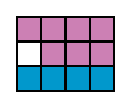
\includegraphics[width=1.7cm]{addition_fraction1} \end{center}
\begin{enumerate}
 \item Explique pourquoi. \label{NbsRatio_entrain2}
 \item En t'inspirant de la question \ref{NbsRatio_entrain2}, écris une égalité illustrant chacune des figures suivantes :
 
 \begin{minipage}[t]{0.28\linewidth}
 \begin{center} Figure 1 \end{center}
 \begin{center} 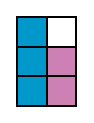
\includegraphics[width=1.1cm]{addition_fraction2} \end{center}
  \end{minipage} \hfill%
 \begin{minipage}[t]{0.38\linewidth}
 \begin{center} Figure 2 \end{center}
 \begin{center} 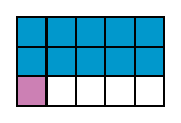
\includegraphics[width=2.6cm]{addition_fraction3} \end{center}
  \end{minipage} \hfill%
 \begin{minipage}[t]{0.3\linewidth}
 \begin{center} Figure 3 \end{center}
 \begin{center} 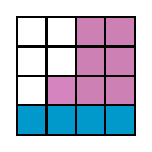
\includegraphics[width=2.1cm]{addition_fraction4} \end{center}
  \end{minipage} \\
 \end{enumerate}
\end{exercice}


\begin{exercice}
Effectue les opérations suivantes et donne le résultat sous la forme d'une fraction irréductible : \\[0.1em]
\begin{colenumerate}{3}
 \item $\dfrac{7}{9} + \dfrac{5}{9}$ ;
 \vspace{0.2cm}
 \item $\dfrac{19}{8} - \dfrac{15}{8}$ ;
 \item $\dfrac{5}{12} + \dfrac{13}{12}$ ;
 \item $\dfrac{9}{11} + \dfrac{7}{11}$ ;
 \item $\dfrac{7}{18} + \dfrac{11}{18}$ ;
  \item $\dfrac{27}{13} - \dfrac{1}{13}$.
 \end{colenumerate}
\end{exercice}


\begin{exercice}
Effectue les opérations suivantes : \\[0.1em]
\begin{colenumerate}{3}
 \item $\dfrac{2}{13} + \dfrac{7}{13}$ ;
 \vspace{0.2cm}
 \item $\dfrac{8}{7} - \dfrac{6}{7}$ ;
 \vspace{0.2cm}
 \item $\dfrac{9}{4} - \dfrac{5}{12}$ ;
 \item $\dfrac{1}{2} + \dfrac{1}{4}$ ;
 \item $\dfrac{1}{3} - \dfrac{1}{6}$ ;
 \item $\dfrac{13}{14} + \dfrac{5}{7}$ ;
 \item $\dfrac{2}{3} - \dfrac{1}{18}$ ;
 \item $\dfrac{8}{5} - \dfrac{16}{10}$ ;
  \item $\dfrac{5}{6} + \dfrac{5}{12}$.
 \end{colenumerate}
\end{exercice}


\begin{exercice}
Effectue les opérations suivantes : \\[0.1em]
\begin{colenumerate}{3}
 \item $4 - \dfrac{3}{2}$ ;
 \vspace{0.2cm}
 \item $2 + \dfrac{1}{3}$ ;
 \vspace{0.2cm}
 \item $\dfrac{9}{4} - 1$ ;
 \item $7 + \dfrac{1}{4}$ ;
 \item $\dfrac{16}{3} - 3$ ;
 \item $4 + \dfrac{5}{7}$ ;
 \item $6 - \dfrac{5}{3} - \dfrac{5}{6}$ ;
 \item $2 + \dfrac{3}{4} + \dfrac{7}{2}$ ;
  \item $7 - \dfrac{9}{5} - \dfrac{13}{25}$.
 \end{colenumerate}
\end{exercice}


\begin{exercice}
Effectue les opérations suivantes : \\[0.1em]
\begin{colenumerate}{3}
 \item $\dfrac{4}{21} + \dfrac{1}{3}$ ;
 \vspace{0.2cm}
 \item $\dfrac{2}{7} - \dfrac{6}{35}$ ;
 \vspace{0.2cm}
 \item $\dfrac{9}{80} - \dfrac{1}{10}$ ;
 \item $\dfrac{1}{8} + \dfrac{5}{56}$ ;
 \item $\dfrac{3}{2} + \dfrac{1}{5}$ ;
 \item $\dfrac{4}{3} + \dfrac{5}{7}$ ;
 \item $\dfrac{1}{5} - \dfrac{1}{4}$ ;
 \item $\dfrac{4}{15} - \dfrac{3}{2}$ ;
  \item $\dfrac{1}{6} + 1$.
 \end{colenumerate}
\end{exercice}


\begin{exercice}
Dans chacun des cas suivants, calcule la valeur de $a + b -  c$ : 
\begin{enumerate}
 \item $a = \dfrac{1}{2}$ ; $b = \dfrac{3}{4}$ ; $c = \dfrac{1}{4}$ ;
  \vspace{0.2cm}
 \item $a = \dfrac{7}{6}$ ; $b = \dfrac{10}{3}$ ; $c = \dfrac{5}{6}$ ;
  \vspace{0.2cm}
 \item $a = \dfrac{1}{3}$ ; $b = \dfrac{1}{9}$ ; $c = \dfrac{1}{27}$ ;
  \vspace{0.2cm}
 \item $a = \dfrac{2}{5}$ ; $b = \dfrac{13}{15}$ ; $c = \dfrac{2}{5}$.
 \end{enumerate}
\end{exercice}


\begin{exercice}[Étonnant !]
\begin{enumerate}
 \item Calcule : $\dfrac{1}{2} + \dfrac{1}{4}$ ;
  \vspace{0.2cm}
 \item Calcule : $\dfrac{1}{2} + \dfrac{1}{4} + \dfrac{1}{8}$ ;
  \vspace{0.2cm}
 \item Calcule : $\dfrac{1}{2} + \dfrac{1}{4} + \dfrac{1}{8} + \dfrac{1}{16}$ ;
  \vspace{0.2cm}
 \item Sans calculer, essaie de deviner la valeur de $\dfrac{1}{2} + \dfrac{1}{4} + \dfrac{1}{8} + \dfrac{1}{16} + \dfrac{1}{32} + \dfrac{1}{64}$ puis vérifie.
 \end{enumerate}
\end{exercice}


\begin{exercice}
Jimmy a mangé $\dfrac{1}{4}$ d'un gâteau. Élise a mangé $\dfrac{3}{8}$ du même gâteau.
\begin{enumerate}
 \item Quelle part du gâteau ont-ils mangée à eux deux ?
 \item Quelle part du gâteau reste-t-il ?
 \end{enumerate}
\end{exercice}


\begin{exercice}[Jeu vidéo]
Trois frères veulent acheter ensemble un jeu vidéo. Le premier ne possède que les $\dfrac{3}{5}$ du prix de ce jeu vidéo, le deuxième n'en possède que les $\dfrac{4}{15}$ et le troisième seulement $\dfrac{1}{3}$. 
\begin{enumerate}
 \item Ont-ils assez d'argent pour acheter ce jeu vidéo ?
 \item Peuvent-ils acheter un second jeu vidéo de même prix ?
 \end{enumerate}
\end{exercice}


\begin{exercice}[Triangle]
$ABC$ est un triangle isocèle en $A$ tel que $AB = \dfrac{5}{7}\,\,BC$ . Quelle fraction de $BC$ représente son périmètre ?
\end{exercice}


\begin{exercice}[Pyramide]
Recopie puis complète la pyramide suivante sachant que le nombre contenu dans une case est la somme des nombres contenus dans les deux cases situées en dessous de lui :
\begin{center} $\boxed{\phantom{\dfrac{16}{42} \dfrac{16}{42} \dfrac{16}{42}}}$ \end{center}
\vspace{-0.72cm}
\begin{center} \boxed{\phantom{\dfrac{16}{42} \dfrac{16}{42} \dfrac{16}{42}}} \negthinspace \boxed{\phantom{\dfrac{16}{42} \dfrac{16}{42} \dfrac{16}{42}}} \end{center}
\vspace{-0.8cm}
\begin{center} \boxed{\phantom{\dfrac{16}{42} \dfrac{16}{42} \dfrac{16}{42}}} \negthinspace \boxed{\phantom{\dfrac{16}{42}} \dfrac{16}{42} \phantom{\dfrac{16}{42}}} \negthinspace  \boxed{\phantom{\dfrac{16}{42} \dfrac{16}{42} \dfrac{16}{42}}} \end{center}
\vspace{-0.79cm}
\begin{center} \negthinspace \boxed{\phantom{!\dfrac{16}{42}} \dfrac{1}{3} \phantom{!\dfrac{16}{42}}} \negthinspace \boxed{\phantom{\dfrac{16}{42}} \dfrac{1}{21} \phantom{\dfrac{16}{42}}} \negthinspace \boxed{\phantom{\dfrac{16}{42} \dfrac{16}{42} \dfrac{16}{42}}} \negthinspace \boxed{\phantom{!\dfrac{16}{42}} \dfrac{2}{3} \phantom{!\dfrac{16}{42}}} \end{center}
\vspace{-0.69cm}
\end{exercice}

%%%%%%%%%%%%%%%%%%%%%%%%%%%%%%%%%%%%%%%%%%%%%%%%%%%%%%%%%%%%%%%%%%%%%%%%